
\documentclass[hyperref={pdfpagelabels=false},ngerman]{beamer}

% stop font warning
\let\Tiny=\tiny
\providecommand\thispdfpagelabel[1]{}

\usepackage[english]{babel}
\usepackage{lmodern}
\usepackage[T1]{fontenc}
\usepackage[utf8]{inputenc}
\usepackage{graphicx,import}
\usepackage{feynmp}
\DeclareGraphicsRule{*}{mps}{*}{} 
\DeclareGraphicsExtensions{.pdf}
\usepackage{amsmath,amssymb,amstext,amsfonts} % mathrsfs
\usepackage{array,booktabs,tabularx}
\usepackage{tikz,tikz-uml,pgf-pie}
\usetikzlibrary{shapes,calc,arrows,positioning}
\tikzstyle{block} = [rectangle, draw, text width=7em, text centered, minimum height=2em]
\tikzstyle{arrow} = [draw, -latex, thick]
\tikzstyle{arrow2} = [draw, latex-latex, thick]
\tikzstyle{quark}  = [rectangle, draw, fill=yellow, minimum width=2em, text centered, minimum height=2em]
\tikzstyle{lepton} = [rectangle, draw, fill=red!50, minimum width=2em, text centered, minimum height=2em]
\tikzstyle{gauge}  = [circle   , draw, fill=green , minimum size=2em, inner sep=0pt, text centered]
\tikzstyle{scalar} = [diamond  , draw, fill=blue!40, minimum width=2.3em, text centered, minimum height=2.3em, inner sep=0pt]
\tikzstyle{goldstone} = [diamond, draw, dashed, fill=blue!30, minimum width=2.3em, text centered, minimum height=2.3em, inner sep=0pt]
\tikzstyle{squark}   = [diamond, draw, fill=yellow, minimum width=2.3em, text centered, minimum height=2.3em, inner sep=0pt]
\tikzstyle{slepton}  = [diamond, draw, fill=red!50, minimum width=2.3em, text centered, minimum height=2.3em, inner sep=0pt]
\tikzstyle{gaugino}  = [rectangle, draw, fill=green , minimum size=2em, inner sep=0pt, text centered]
\tikzstyle{higgsino} = [rectangle, draw, fill=blue!40  , minimum width=2em, text centered, minimum height=2em]
\tikzstyle{inert}    = [diamond  , draw, fill=teal!80, minimum width=2.3em, text centered, minimum height=2.3em, inner sep=0pt]
\tikzstyle{inertino} = [rectangle, draw, fill=teal!80, minimum width=2em, text centered, minimum height=2em]
\tikzstyle{phantom}  = [rectangle, minimum width=2em, text centered, minimum height=2em]
\usepackage{slashed}
\usepackage{fixltx2e} % textsubscript
\usepackage{multirow}
\usepackage{tcolorbox}
\usepackage{pifont}
\usepackage{xspace}
\usepackage{hyperref}
\hypersetup{colorlinks,linkcolor=,urlcolor=blue}
\usepackage{listings}
\lstset{breaklines=true,
  breakatwhitespace=true,
%  numbers=left,
  numberstyle=\tiny,
  stepnumber=1,
  basicstyle=\ttfamily\footnotesize,
  commentstyle=\ttfamily\color{gray},
  postbreak={\mbox{{$\hookrightarrow$}}\space\space},
  breakindent=10pt,
  breakautoindent=false,
  showspaces=false,
  showstringspaces=false,
  frame=single}

\definecolor{darkgreen}{RGB}{0,176,0}

\newcommand{\cmark}{\ding{51}}%
\newcommand{\xmark}{\ding{55}}%
\newcommand{\fmfvcenter}[1]{\;\vcenter{\hbox{\fmfreuse{#1}}}\;}
\newcommand{\eh}[1]{\,\mathsf{#1}}
\newcommand{\ok}{\textcolor{darkgreen}{\cmark}}
\newcommand{\notok}{\textcolor{red}{\xmark}}
\newcommand{\maybe}{\textcolor{gray}{\cmark}}
\newcommand{\meh}{\textcolor{gray}{\textbf{\huge\lower.1em\hbox{-}}}}
\newcommand{\Lagr}{\mathcal{L}}
\newcommand{\MS}{\ensuremath{M_S}}
\newcommand{\mathi}{\mathsf{i}}
\newcommand{\mycite}[1]{\ensuremath{\text{\textcolor{darkgray}{\tiny [#1]}}}}
\newcommand{\bigcite}[1]{\textcolor{darkgray}{[#1]}}
\newcommand{\dimrep}[1]{\mathbf{#1}}
\newcommand{\dimrepadj}[1]{\mathbf{\overline{#1}}}
\newcommand{\ESSM}{E\textsubscript{6}SSM}
\newcommand{\CESSM}{CE\textsubscript{6}SSM}
\DeclareMathOperator{\tildeRe}{\widetilde Re}
\DeclareMathOperator{\sign}{sign}
\DeclareMathOperator{\re}{Re}
\DeclareMathOperator{\im}{Im}
\renewcommand{\emph}{\textbf}
\newcommand{\dd}{\mathsf{d}}
\newcommand{\myurl}[1]{\href{#1}{#1}}
\newcommand{\Superpot}{\mathcal{W}}
\newcommand{\SuperField}[1]{#1}
\newcommand{\ConjSuperField}[1]{\bar{#1}}
\newcommand{\UY}{\ensuremath{U(1)_{Y}}}
\newcommand{\UN}{\ensuremath{U(1)_{N}}}
\newcommand{\Uem}{\ensuremath{U(1)_\text{em}}}
\newcommand{\SUL}{\ensuremath{SU(2)_\text{L}}}
\newcommand{\SUc}{\ensuremath{SU(3)_\text{c}}}
\newcommand{\SOten}{\ensuremath{{SO(10)}}}
\newcommand{\comma}{,}
\newcommand{\DRbar}{\ensuremath{\overline{\text{DR}}}}
\newcommand{\DRbarp}{\ensuremath{\overline{\text{DR}}'}}
\newcommand{\MSbar}{\ensuremath{\overline{\text{MS}}}}
\newcommand{\SM}{\ensuremath{\text{SM}}}
\newcommand{\MSSM}{\ensuremath{\text{MSSM}}}
\newcommand{\pole}{\ensuremath{\text{pole}}}
\newcommand{\tree}{\ensuremath{\text{tree}}}
\newcommand{\fsstar}{\textbf{*}}
\newcommand{\fs}{\texttt{FlexibleSUSY}\xspace}
\newcommand{\fsh}{\texttt{FS+H}\xspace}
\newcommand{\feft}{\texttt{FlexibleEFTHiggs}\xspace}
\newcommand{\hssusy}{\texttt{HSSUSY}\xspace}
\newcommand{\Himalaya}{\texttt{Himalaya}\xspace}
\newcommand{\FH}{\texttt{FeynHiggs}\xspace}
\newcommand{\SPheno}{\texttt{SPheno}\xspace}
\newcommand{\Zv}{\ensuremath{\backslash\mkern-11.0mu{Z_3}}}
\newcommand{\downrightknickarrow}{\mathrel{\scalebox{1.3}{\rotatebox[origin=c]{180}{$\Lsh$}}}}
\newcommand{\threelinebrace}{$\left. \begin{array}{c} \\ \\ \\ \end{array} \right\rbrace$}
\newcommand{\fivelinebrace}{$\left. \begin{array}{c} \\ \\ \\ \\ \\ \end{array} \right\rbrace$}
\newcommand{\twolinebrace}{$\left. \begin{array}{c} \\ \\ \end{array} \right\rbrace$}
\newcommand{\elevenlinebrace}{$\left. \begin{array}{c} \\ \\ \\ \\ \\ \\ \\ \\ \\ \\ \\ \end{array} \right\rbrace$}
\newcommand{\at}{\alpha_t}
\newcommand{\ab}{\alpha_b}
\newcommand{\atau}{\alpha_\tau}
\newcommand{\as}{\alpha_s}
\newcommand{\aem}{\alpha_\text{em}}
\newcommand{\GeV}{\eh{GeV}}
\newcommand{\TeV}{\eh{TeV}}

% set look of slides
\usetheme{Madrid}
\useoutertheme{default}
\useinnertheme{circles}
\usecolortheme{default}
\beamertemplatenavigationsymbolsempty % keine Navigationselemente
\setbeamersize{text margin left = 1cm, text margin right = 1cm}

% define footer
\makeatletter
\setbeamertemplate{footline}
{
  \hfill\hbox{\insertframenumber{} / \inserttotalframenumber\hspace*{4pt}}%
  \vskip3pt%
}
\makeatother
\usecolortheme{tud}

\title{Precise Higgs mass predictions in the (N)MSSM}

\author[Alexander Voigt]{Alexander Voigt}

\date{SUSY-2018\\[1em]
  23--27/07/2018}

% \institute[Aachen]{RWTH Aachen}
\subject{FlexibleSUSY,MSSM,Higgs,FlexibleEFTHiggs}
\keywords{FlexibleSUSY,MSSM,Higgs,FlexibleEFTHiggs}

%%%%%%%%%%%%%%%%%%%%%%%%%%%%%%%%%%%%%%%%%%%%%%%%%%%%%%%%%%%%%%%%%%%%%%%%%%%%%

\begin{document}

%%%%%%%%%%%%%%%%%%%%%%%%%%%%%%%%%%%%%%%%%%%%%%%%%%%%%%%%%%%%%%%%%%%%%%%%%%%%%

% Savebox which contains the the Feynman rules
\newsavebox{\feynmanrules}
\sbox{\feynmanrules}{
\begin{fmffile}{Feynman/higgs} % file name and path
  \fmfset{thin}{.8pt}
  \fmfset{wiggly_len}{5mm}
  \fmfset{dash_len}{2.5mm}
  \fmfset{dot_size}{1thick}
  \fmfset{arrow_len}{2.5mm}
  \fmfset{curly_len}{2.5mm}

\begin{fmfgraph*}(60,60)
  \fmfkeep{hX}
  \fmfleft{v1}
  \fmfright{v2}
  \fmf{higgs}{v1,c1}
  \fmf{higgs}{c2,v2}
  \fmf{quark,left,tension=0.5,label=$X$}{c1,c2}
  \fmf{quark,left,tension=0.5}{c2,c1}
\end{fmfgraph*}

\begin{fmfgraph*}(60,60)
  \fmfkeep{htop}
  \fmfleft{v1}
  \fmfright{v2}
  \fmf{higgs}{v1,c1}
  \fmf{higgs}{c2,v2}
  \fmf{quark,left,tension=0.5,label=$t$}{c1,c2}
  \fmf{quark,left,tension=0.5}{c2,c1}
\end{fmfgraph*}

\begin{fmfgraph*}(60,60)
  \fmfkeep{hstop}
  \fmfleft{v1}
  \fmfright{v2}
  \fmf{higgs}{v1,c1}
  \fmf{higgs}{c2,v2}
  \fmf{scalar,left,tension=0.5,label=$\tilde{t}_i$}{c1,c2}
  \fmf{scalar,left,tension=0.5}{c2,c1}
\end{fmfgraph*}

\begin{fmfgraph*}(60,60)
  \fmfkeep{hstopA}
  \fmfleft{v1}
  \fmfright{v2}
  \fmf{higgs}{v1,c,v2}
  \fmf{scalar,right,tension=0.8,label=$\tilde{t}_i$}{c,c}
\end{fmfgraph*}

\begin{fmfgraph*}(60,60)
  \fmfkeep{htoptad}
  \fmfleft{v1}
  \fmfright{v2}
  \fmftop{t1}
  \fmf{higgs}{v1,c,v2}
  \fmffreeze
  \fmf{higgs}{c,c1}
  \fmf{quark,right,tension=0.3,label=$t$}{c1,c2}
  \fmf{quark,right,tension=0.3}{c2,c1}
  \fmf{phantom,tension=10}{c2,t1}
\end{fmfgraph*}

\begin{fmfgraph*}(60,60)
  \fmfkeep{hstoptad}
  \fmfleft{v1}
  \fmfright{v2}
  \fmftop{t1}
  \fmf{higgs}{v1,c,v2}
  \fmffreeze
  \fmf{higgs}{c,c1}
  \fmf{scalar,right,tension=0.3,label=$\tilde{t}_i$}{c1,c2}
  \fmf{scalar,right,tension=0.3}{c2,c1}
  \fmf{phantom,tension=10}{c2,t1}
\end{fmfgraph*}
\end{fmffile}
}

%%%%%%%%%%%%%%%%%%%%%%%%%%%%%%%%%%%%%%%%
\begin{frame}[plain]
  \tikz [remember picture,overlay]
  \node at
    ([yshift=1.3cm,xshift=4cm]current page.south)
    {\includegraphics[height=2cm]{images/RWTH_Logo}};
  \titlepage  
\end{frame}

%%%%%%%%%%%%%%%%%%%%%%%%%%%%%%%%%%%%%%%%
\begin{frame}{Contents}
  \tableofcontents
\end{frame}

%%%%%%%%%%%%%%%%%%%%%%%%%%%%%%%%%%%%%%%%

\begin{frame}{Current limits on SUSY particle masses}
  \begin{center}
    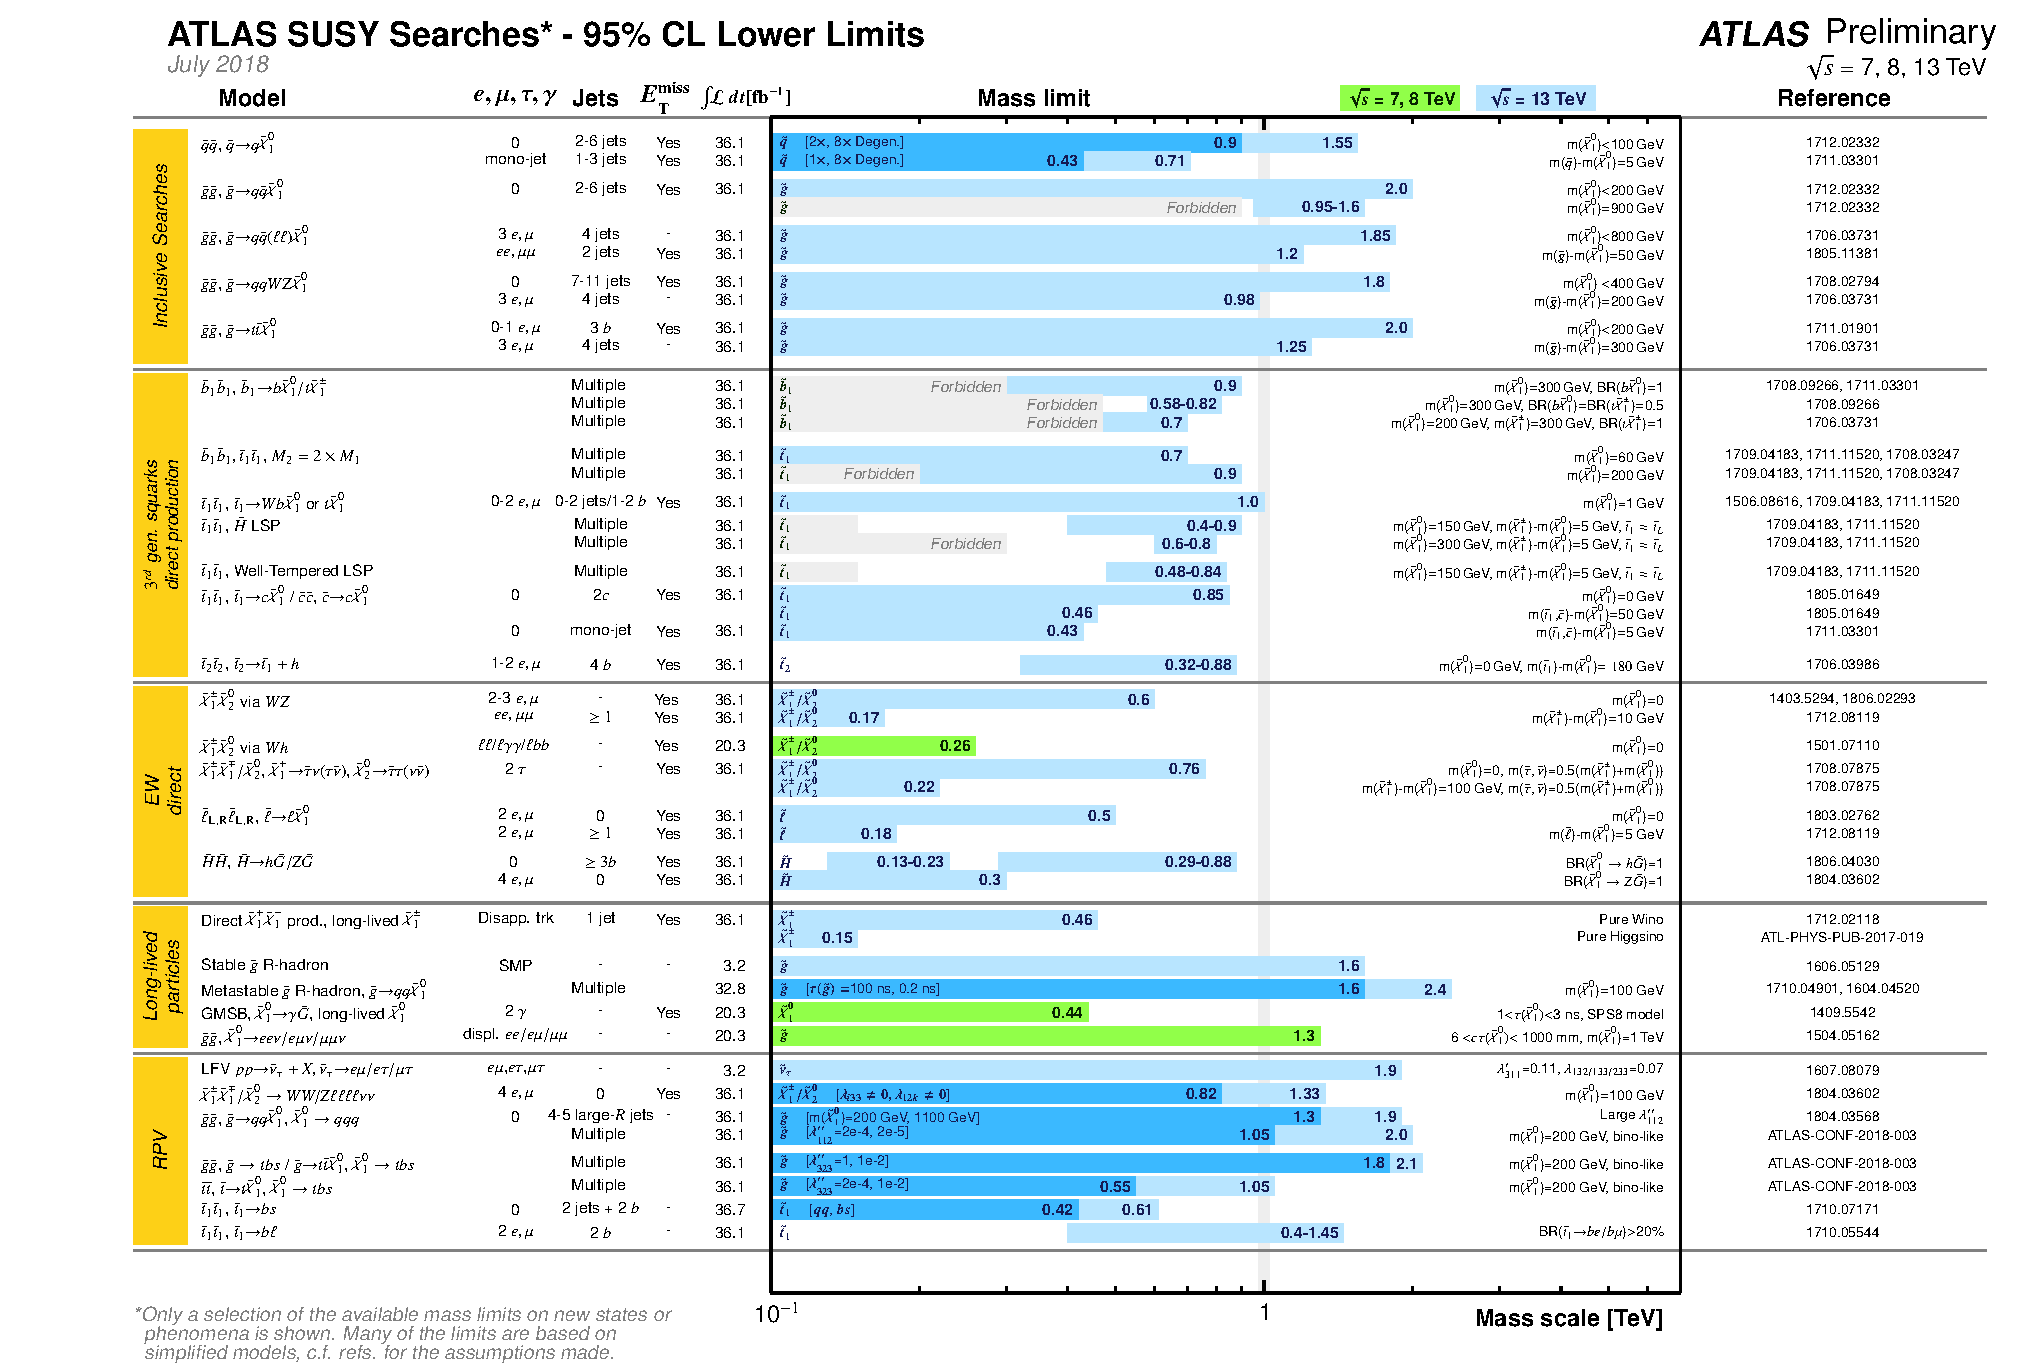
\includegraphics[width=\textwidth]{images/ATLAS_SUSY_Summary}
  \end{center}
\end{frame}

\section{Higgs mass calculation}
\subsection{at fixed loop order}

\begin{frame}{Contents}
  \tableofcontents[
  currentsection,
  currentsubsection,
  subsectionstyle=show/shaded/hide]  
\end{frame}

% \begin{frame}{Fixed-order calculation}
%   \begin{center}
%   \begin{tikzpicture}
%     \path[arrow] (0,0) -- (0,5) node[left]{$Q$};
%     \draw[thick,darkgreen] (0,4) node[left]{$M_S$} -- node[above = 0.5cm,black]{MSSM} (3,4) node[right,black,text width=8cm]{
%       $M_h^2$ at $O(\text{1L} + (\at+\ab)\as + (\at+\ab)^2)$\\ \ \ \ \ \ + $O(\atau^2) + O((\at + \ab)\as^2)$};
%     \draw[thick,darkgreen] (0,1) node[left]{$M_Z$} -- node[above = 1.2cm,black]{MSSM} node[below = 0.5cm,black]{SM(5)} (3,1) node[right,black,text width=8cm]{
%       $y_{t,b}$ at $O(\text{1L} + \as^2)$, $v$ at 1L, \\ $g_3$ at $O(\text{1L} + \as^2 + (\at + \ab)\as)$};
%     \path[arrow,latex-latex,blue] (-1,1) -- node[above,rotate=90]{3L RGEs} (-1,4);
%   \end{tikzpicture}
%   \end{center}
%   $M_h^2$: \mycite{0105096, 0112177, 0212132, 0206101, 0305127, 1708.05720}\\
%   $y_{t,b}$: \mycite{0210258, 0507139, 0707.0650, 0912.4652},
%   $g_3$: \mycite{0509048, 0810.5101, 1009.5455}\\
%   $\aem$: \mycite{1411.7040}, 
%   $\beta_i$: \mycite{0308231, 0408128}
% \end{frame}

\begin{frame}{Higgs mass calculation at fixed loop order}
  % \emph{Idea:} Integrate out SUSY particles at $\MS$ (expand in $v^2/\MS^2$) \\
  % $\Rightarrow$ $\lambda(\MS)$ is fixed by the MSSM \\
  % $\Rightarrow$ effectively: separation of scales $\MS$ and $M_t$.
  \begin{center}
    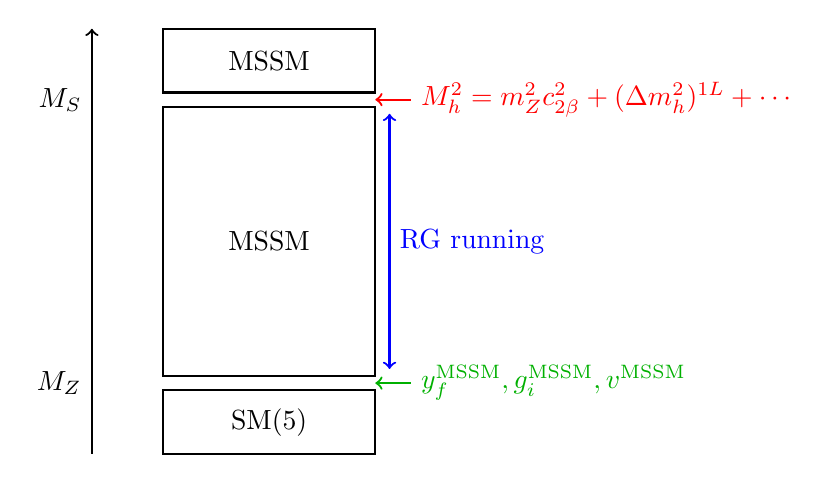
\begin{tikzpicture}[scale=0.9]
      \draw[->, thick] (0,0) -- (0,1) node[left]{$M_Z$} -- (0,5) node[left]{$\MS$} -- (0,6);
      \draw[thick] (1,0)   rectangle node{SM(5)} (4,0.9);
      \draw[thick] (1,1.1) rectangle node{MSSM}  (4,4.9);
      \draw[thick] (1,5.1) rectangle node{MSSM}  (4,6);
      \draw[<-, thick, red] (4,5) -- (4.5,5) node[right]{$M_h^2 = m_Z^2 c_{2\beta}^2 + (\Delta m_h^2)^{1L} + \cdots$};
      \draw[<-, thick, darkgreen] (4,1) -- (4.5,1) node[right]{$y_f^\MSSM, g_i^\MSSM, v^\MSSM$};
      \draw[<->, thick, blue] (4.2,1.2) -- node[right]{RG running} (4.2,4.8);
    \end{tikzpicture}
  \end{center}
\end{frame}

\begin{frame}{Known/unknown fixed order \DRbarp\ loop corrections}
  Loop corrections in the determination of the running MSSM
    parameters $y_f^\MSSM$, $g_i^\MSSM$:
    \begin{align*}
      y_t^\MSSM &= \frac{\sqrt{2}\,M_t}{v_u}
      \Big[1 + \hbar(\textcolor{darkgreen}{\text{full}})
      + \hbar^2(\textcolor{darkgreen}{\as^2} + \textcolor{red}{\at\as} + \textcolor{red}{\at^2})
      + \cdots \Big] \\
      \as^\MSSM &= \as^{\SM(5)}
      \Big[1 + \hbar(\textcolor{darkgreen}{\text{full}})
      + \hbar^2(\textcolor{darkgreen}{\as^2} + \textcolor{darkgreen}{\at\as} + \textcolor{darkgreen}{\ab\as})
      + \cdots \Big]
    \end{align*}
    Loop corrections to $M_h^2$ in the MSSM:
    \begin{align*}
      M_h^2 &= m_h^2 + \hbar(\textcolor{darkgreen}{\text{full}})
      + \hbar^2\Big[ m_t^2(\textcolor{darkgreen}{\at\as} + \textcolor{darkgreen}{\at^2} + \cdots)
      + \textcolor{red}{m_Z^2\aem^2}
      + \cdots\Big]\\
      &\quad + \hbar^3\Big[ m_t^2(\textcolor{darkgreen}{\at\as^2} + \textcolor{red}{\at^2\as} + \textcolor{red}{\at^3})
      + \cdots\Big]
    \end{align*}
    \mycite{0105096, 0112177, 0212132, 0206101, 0305127, 1005.5709, 1708.05720}
\end{frame}

\begin{frame}{Uncertainty of the fixed order \DRbarp\ calculation}
  \begin{center}
    \includegraphics[width=0.7\textwidth]{{{plots/SOFTSUSY/SS_TB-20_Xt--sqrt6}}}
  \end{center}
\end{frame}

\begin{frame}{Summary of fixed loop order calculation}
  Typical order of magnitude of loop contributions (depends on
  parameter scenario):
  \begin{align*}
    M_h &= m_h + \Delta m_h^{1L} + \Delta m_h^{2L} + \Delta m_h^{3L} + \cdots \\
    &\approx [91 + O(20\ldots 30) + O(2\ldots 4) + O(1\ldots 2)] \eh{GeV}
  \end{align*}
  \emph{Advantages:}
  \begin{itemize}
  \item includes logarithmic, non-logarithmic and suppressed terms of
    the order $O(v^2/\MS^2)$ at fixed loop order
  \item precise prediction if $\MS \sim m_t$
  \end{itemize}
  \emph{Problem:}
  \begin{itemize}
  \item large logarithmic corrections, if $\MS \gg m_t$ \\
    $\Rightarrow$ slow convergence of perturbation series \\
    $\Rightarrow$ large theoretical uncertainty, ($1$--$2\eh{GeV}$, or
    more) \\
    recall: $M_h^{\text{exp}} = (125.09 \pm 0.24)\eh{GeV}$
  \end{itemize}
\end{frame}

%%%%%%%%%%%%%%%%%%%%%%%%%%%%%%%%%%%%%%%%

\subsection{in an EFT}

\begin{frame}{Contents}
  \tableofcontents[
  currentsection,
  currentsubsection,
  subsectionstyle=show/shaded/hide]  
\end{frame}

% \begin{frame}{EFT calculation (\texttt{HSSUSY})}
%   \begin{center}
%   \begin{tikzpicture}
%     \path[arrow] (0,0) -- (0,5) node[left]{$Q$};
%     \draw[thick,darkgreen] (0,4) node[left]{$M_S$} -- node[above = 0.5cm,black]{MSSM} (3,4) node[right,black,text width=8cm]{
%       $\lambda$ at $O(\text{1L} + (\at+\ab)\as + (\at+\ab)^2)$\\ \ \ \ \ \ + $O(\atau^2)$};
%     \draw[thick,dashed,darkgreen] (0,2) node[left]{$M_t$} -- (3,2) node[right,black,text width=8cm]{
%       $M_h^2$ at $O(\text{1L} + (\at+\as)\at)$\\ \ \ \ \ \ \ + $O(\at^3 + \at^2\as + \at\as^2)$
%     };
%     \draw[thick,darkgreen] (0,1) node[left]{$M_Z$} -- node[above = 1.5cm,black]{SM} node[below = 0.5cm,black]{SM(5)} (3,1) node[right,black,text width=8cm]{
%       $y_t$ at $O(\text{1L} + \as^2 + \as^3)$, $v$ at 1L, \\ $g_3$ at $O(\text{1L} + \as^2 + \as^3)$};
%     \path[arrow,latex-latex,blue] (-1,1) -- node[above,rotate=90]{3L RGEs} (-1,4);
%   \end{tikzpicture}
%   \end{center}
%   $\lambda$: \mycite{1407.4081, 1504.05200, 1703.08166}
%   $M_h^2$: \mycite{1205.6497, 1504.05200, 1407.4336}\\
%   $y_t$: \mycite{9912391, 1205.2892},
%   $g_3$: \mycite{9305305, 9707474, 9708255, 0004189}\\
%   $\beta_i$: \mycite{1201.5868, 1210.6873, 1212.6829, 1205.2892, 1303.4364}
% \end{frame}

\begin{frame}{Higgs mass calculation in an EFT}
  \emph{Idea:} Integrate out SUSY particles at $\MS$ (expand in $v^2/\MS^2$) \\
  $\Rightarrow$ $\lambda(\MS)$ is fixed by the MSSM \\
  $\Rightarrow$ effectively: separation of scales $\MS$ and $M_t$.
  \begin{center}
    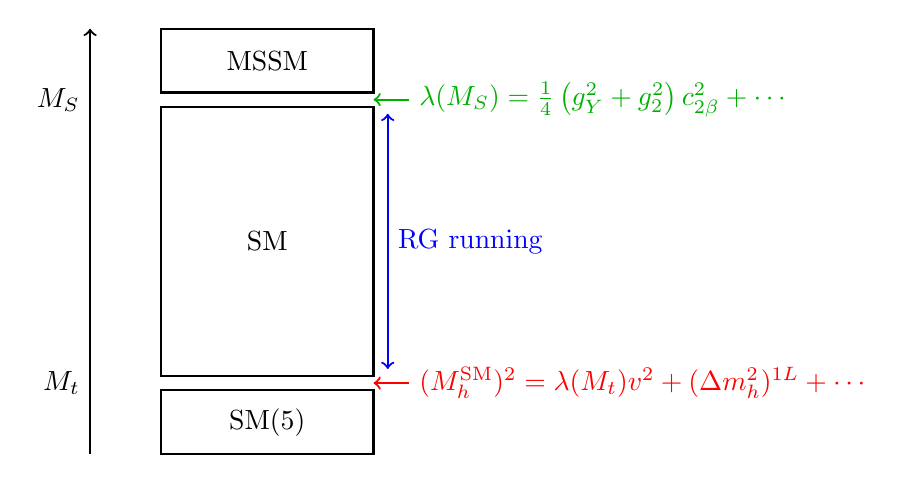
\begin{tikzpicture}[scale=0.9]
      \draw[->, thick] (0,0) -- (0,1) node[left]{$M_t$} -- (0,5) node[left]{$\MS$} -- (0,6);
      \draw[thick] (1,0)   rectangle node{SM(5)} (4,0.9);
      \draw[thick] (1,1.1) rectangle node{SM}    (4,4.9);
      \draw[thick] (1,5.1) rectangle node{MSSM}  (4,6);
      \draw[<-, thick, darkgreen] (4,5) -- (4.5,5) node[right]{$\lambda(\MS) = \frac{1}{4}\left(g_Y^{2} + g_2^2\right) c^2_{2\beta} + \cdots$};
      \draw[<-, thick, red] (4,1) -- (4.5,1) node[right]{$(M_h^\SM)^2 = \lambda(M_t) v^2 + (\Delta m_h^2)^{1L} + \cdots$};
      \draw[<->, thick, blue] (4.2,1.2) -- node[right]{RG running} (4.2,4.8);
    \end{tikzpicture}
  \end{center}
\end{frame}

\begin{frame}{Known/unknown loop corrections in the EFT calculation}
  \emph{SM contributions:}
  \begin{itemize}
  \item Loop corrections in the determination of the running SM
    parameters $y_f^\SM$, $g_i^\SM$:
    \begin{align*}
      y_t^\SM &= \frac{\sqrt{2}\,M_t}{v}
      \Big[1 + \hbar(\textcolor{darkgreen}{\text{full}})
      + \hbar^2(\textcolor{darkgreen}{\as^2} + \textcolor{darkgray}{\at\as} + \textcolor{darkgray}{\at^2})
      + \hbar^3(\textcolor{darkgreen}{\as^3} + \cdots)
      \Big] \\
      \as^\SM &= \as^{\SM(5)}
      \Big[1 + \hbar(\textcolor{darkgreen}{\text{full}})
      + \hbar^2(\textcolor{darkgreen}{\as^2} + \cdots)
      + \hbar^3(\textcolor{darkgreen}{\as^3} + \cdots)
      + \cdots \Big]
    \end{align*}
  \item Loop corrections to $M_h^2$ in the SM:
    \begin{align*}
      M_h^2 &= m_h^2 + \hbar(\textcolor{darkgreen}{\text{full}})
      + \hbar^2\Big[ m_t^2(\textcolor{darkgreen}{\at\as} + \textcolor{darkgreen}{\at^2} + \cdots)
      + \textcolor{darkgray}{m_Z^2\aem^2}
      + \cdots\Big]\\
      &\quad + \hbar^3\Big[ m_t^2(\textcolor{darkgreen}{\at\as^2} + \textcolor{darkgreen}{\at^2\as} + \textcolor{darkgreen}{\at^3})
        + \textcolor{red}{m_Z^2 \aem^3} + \cdots \Big]\\
      &\quad + \hbar^4\Big[ m_t^2(\textcolor{darkgreen}{\at\as^4} + \cdots)
      + \cdots\Big]
    \end{align*}
  \end{itemize}
\end{frame}

\begin{frame}{Known/unknown loop corrections in the EFT calculation}
  \emph{SUSY contributions:} Loop corrections to $\lambda(\MS)$:
  \begin{align*}
      \lambda(\MS) &= \frac{1}{4}(g_Y^2+g_2^2)c_{2\beta}^2 + \hbar(\textcolor{darkgreen}{\text{full}}) \\
      &\quad + \hbar^2\Big[ (\textcolor{darkgreen}{\at^2\as} + \textcolor{darkgreen}{\ab^2\as}
        + \textcolor{darkgreen}{\at^2\ab} + \textcolor{darkgreen}{\at\ab^2} + \textcolor{darkgreen}{\at^3} + \cdots)
      + \textcolor{red}{\aem^3}
      + \cdots\Big]\\
      &\quad + \hbar^3\Big[ (\textcolor{darkgreen}{\at^2\as^2} + \textcolor{red}{\at^3\as} + \textcolor{red}{\at^4})
        + \textcolor{red}{\aem^4} + \cdots \Big]
  \end{align*}
  \emph{Neglected contributions:} Terms of $O(v^2/\MS^2)$
\end{frame}

\begin{frame}{Comparison of fixed-order and EFT approaches}
  \begin{center}
    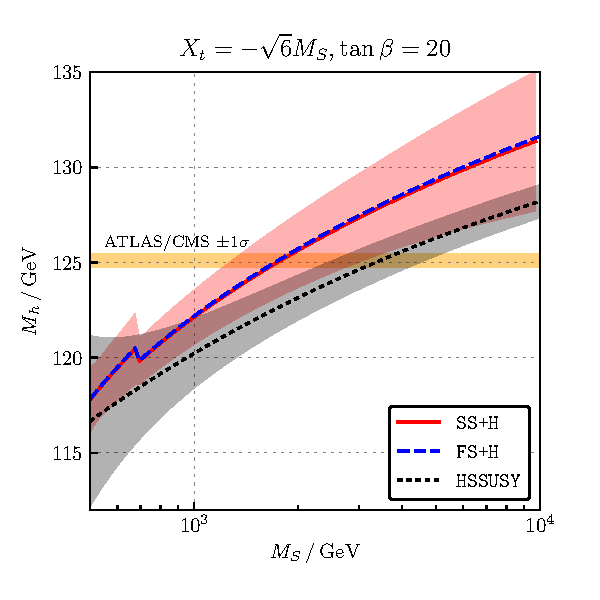
\includegraphics[width=0.7\textwidth]{plots/SOFTSUSY/Mh_MS_TB-20_Xt--sqrt6}
    % \includegraphics[width=0.7\textwidth]{{{plots/uncertainties/Mh_MS_TB-5_Xt-0_FO_EFT}}}
  \end{center}
\end{frame}

\begin{frame}{Summary of EFT approach}
  Typical order of magnitude of loop contributions (depends on
  parameter scenario, here $X_t = 0$, $\MS = 20\eh{TeV}$):
  \begin{align*}
    M_h &= m_h + \Delta m_h^{1L} + \Delta m_h^{2L} + \Delta m_h^{3L} + \cdots \\
    &\approx [O(124) + O(0.5\ldots 1) + O(0.1\ldots 0.2) + O(0.02\ldots 0.04)] \eh{GeV}
  \end{align*}
  \emph{Advantages:}
  \begin{itemize}
  \item large logarithmic fixed order loop corrections are avoided
  \item large logarithms $\propto\ln(M_S/M_t)$ are resummed to all orders
  \end{itemize}
  \emph{Disadvantage:} usually terms $O(v^2/M_S^2)$ are neglected \\
  $\Rightarrow$ imprecise when $v \sim \MS$ \\
  $\Rightarrow$ large theoretical uncertainty when $v \sim \MS$
\end{frame}

\begin{frame}{Summary of fixed-order and EFT approaches}
  \begin{center}
    \begin{tabular}{lcc}
      \toprule
                  & low $\MS$ & high $\MS$ \\
                  & $\MS \lesssim 2\eh{TeV}$ & $\MS \gtrsim 2\eh{TeV}$ \\
      \midrule
      fixed-order & \ok       & \notok     \\
      EFT         & \notok    & \ok        \\
      ? mixed     & \ok       & \ok        \\
      \bottomrule
    \end{tabular}
  \end{center}
  \vspace{2em}
  Q: Can the fixed-order and EFT approaches be combined? \\[1em]
  A: Yes!  \mycite{1312.4937, 1609.00371, 1710.03760}
\end{frame}

%%%%%%%%%%%%%%%%%%%%%%%%%%%%%%%%%%%%%%%%

\subsection{in a mixed fixed-order/EFT calculation}

\begin{frame}{Contents}
  \tableofcontents[
  currentsection,
  currentsubsection,
  subsectionstyle=show/shaded/hide]  
\end{frame}

\begin{frame}{Mixed fixed-order/EFT calculations}
  \emph{Goal:} resum large logarithms \emph{and} include suppressed
  $O(v^2/\MS^2)$ terms
  \\[2em]
  \emph{Two known approaches:}
  \begin{itemize}
  \item FeynHiggs \mycite{1312.4937, 1706.00346, 1805.00867}: Replace logs from
    fixed-order calculation by resummed logs
    \begin{align*}
      M_h^2 = (M_h^2)_{\text{fixed-order}} - (M_h^2)_{\text{logs}} + (M_h^2)_{\text{resummed logs}}
    \end{align*}
  \item FlexibleEFTHiggs \mycite{1609.00371, 1710.03760}: Incorporate
    $O(v^2/\MS^2)$ terms into $\lambda$ by using the matching
    condition
    \begin{align*}
      (M_h^2)_{\SM} \overset{!}{=} (M_h^2)_{\MSSM} \qquad \text{at 1L level at } Q = \MS
    \end{align*}
  \end{itemize}
\end{frame}

\begin{frame}{FlexibleEFTHiggs approach \mycite{1609.00371, 1710.03760}}
  \emph{Idea:}
  Determine $\lambda(\MS)$ from the condition
  \begin{align*}
    (M_h^2)_{\SM} \equiv \lambda(\MS) v^2 + (\Delta m_h^2)_{\SM} \overset{!}{=} (M_h^2)_{\MSSM} , \qquad Q = \MS
  \end{align*}
  \begin{center}
    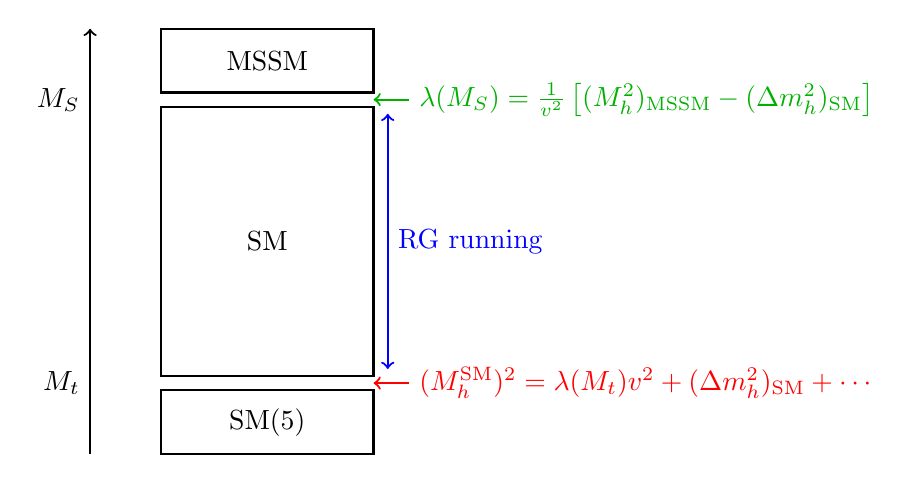
\begin{tikzpicture}[scale=0.9]
      \draw[->, thick] (0,0) -- (0,1) node[left]{$M_t$} -- (0,5) node[left]{$\MS$} -- (0,6);
      \draw[thick] (1,0)   rectangle node{SM(5)} (4,0.9);
      \draw[thick] (1,1.1) rectangle node{SM}    (4,4.9);
      \draw[thick] (1,5.1) rectangle node{MSSM}  (4,6);
      \draw[<-, thick, darkgreen] (4,5) -- (4.5,5) node[right]{$\lambda(\MS) = \frac{1}{v^2}\left[(M_h^2)_{\MSSM} - (\Delta m_h^2)_{\SM}\right]$};
      \draw[<-, thick, red] (4,1) -- (4.5,1) node[right]{$(M_h^\SM)^2 = \lambda(M_t) v^2 + (\Delta m_h^2)_{\SM} + \cdots$};
      \draw[<->, thick, blue] (4.2,1.2) -- node[right]{RG running} (4.2,4.8);
    \end{tikzpicture}
  \end{center}
\end{frame}

\begin{frame}{Comparison of the three approaches in the MSSM}
  \begin{center}
    \includegraphics[width=0.49\textwidth]{{{plots/uncertainties/Mh_MS_TB-5_Xt-0}}}
    \hfill
    \includegraphics[width=0.49\textwidth]{{{plots/uncertainties/DMh_MS_TB-5_Xt-0_alt}}}
  \end{center}
\end{frame}

\begin{frame}{Comparison of the three approaches in the NMSSM}
  \begin{center}
    \includegraphics[width=0.35\textwidth]{{{plots/NMSSMEFTHiggs/DMh_MS_TB-5_Xt-0_lam-0.1_kap-0.1}}}%\hfill
    \includegraphics[width=0.35\textwidth]{{{plots/NMSSMEFTHiggs/DMh_MS_TB-5_Xt-0_lam-0.3_kap-0.3}}}\\
    \includegraphics[width=0.35\textwidth]{{{plots/NMSSMEFTHiggs/DMh_MS_TB-5_Xt--2_lam-0.1_kap-0.1}}}%\hfill
    \includegraphics[width=0.35\textwidth]{{{plots/NMSSMEFTHiggs/DMh_MS_TB-5_Xt--2_lam-0.3_kap-0.3}}}
  \end{center}
\end{frame}

\begin{frame}{Summary FlexibleEFTHiggs approach}
  \begin{align*}
    (M_h^2)_{\SM} &= (M_h^2)_{\MSSM} \qquad \text{at 1L, } Q = \MS
  \end{align*}
  \emph{Advantages:}
  \begin{itemize}
  \item large logarithms $\propto\ln(M_S/M_t)$ are resummed to all orders
  \item all suppressed terms $O(v^2/\MS^2)$ are incorporated in $\lambda$
  \end{itemize}
  \vspace{1em}
  \textcolor{darkgreen}{$\Rightarrow$ FlexibleEFTHiggs leads to a
    correct Higgs mass prediction at the full 1-loop level (including
    suppressed terms) with additional NLL resummation.}\\
  \vspace{1em}
  \emph{Disadvantage:}
  \begin{itemize}
  \item tricky to extend to 2-loop accuracy (work in progress)
  \end{itemize}
\end{frame}

%%%%%%%%%%%%%%%%%%%%%%%%%%%%%%%%%%%%%%%%

\section{Current status of Higgs mass prediction in the MSSM}

\begin{frame}{Current status of high precision calculation in the MSSM}
  Currently most precise tools: \fsh (3-loop fixed order
  \mycite{1708.05720}), \hssusy (2-loop EFT \mycite{1710.03760}),
  \FH (2-loop mixed \mycite{1312.4937, 1608.01880, 1706.00346}),
  \SPheno (2-loop$^*$ mixed \mycite{1703.03267})
  \begin{center}
    \includegraphics[width=0.49\textwidth]{{{plots/uncertainties/DMh_MS_TB-5_Xt-0}}}\hfill
    \includegraphics[width=0.49\textwidth]{{{plots/uncertainties/DMh_MS_TB-5_Xt--2}}}
%    \includegraphics[width=0.49\textwidth]{{{plots/uncertainties/DMh_Xt_TB-5_MS-5000}}}
  \end{center}
  $\MS \lesssim 2\eh{TeV}$ $\Rightarrow$ \fsh more accurate than \hssusy\\
  $\MS \gtrsim 2\eh{TeV}$ $\Rightarrow$ \fsh less accurate than \hssusy
\end{frame}

%%%%%%%%%%%%%%%%%%%%%%%%%%%%%%%%%%%%%%%%

\section{Summary}

\begin{frame}{Summary}
  \emph{Supersymmetry} is still viable, but LHC continuously excludes
  light SUSY scenarios\\[1em]
  %
  \emph{Approaches to calculate $M_h$:}
  \begin{center}
    \begin{tabular}{lcc}
      \toprule
                               & low $\MS$ & high $\MS$ \\
                               & $\MS \lesssim 2\eh{TeV}$ & $\MS \gtrsim 2\eh{TeV}$ \\
      \midrule
      fixed-order              & \ok       & \notok     \\
      EFT                      & \notok    & \ok        \\
      mixed (FlexibleEFTHiggs) & \ok       & \ok        \\
      \bottomrule
    \end{tabular}
  \end{center}
  %
  \emph{FlexibleEFTHiggs:}
  \begin{itemize}
  \item full NLO + NLL resummation
  \item can be applied to \emph{any} BSM model (SUSY or non-SUSY)
  \item can be easily automatized
  \item tricky to extend to 2-loop level (work in progress)
  \end{itemize}
\end{frame}

%%%%%%%%%%%%%%%%%%%%%%%%%%%%%%%%%%%%%%%%
% backup slides
%%%%%%%%%%%%%%%%%%%%%%%%%%%%%%%%%%%%%%%%

\begin{frame}[noframenumbering]
  \begin{center}
    \Huge Backup
  \end{center}
\end{frame}

%%%%%%%%%%%%%%%%%%%%%%%%%%%%%%%%%%%%%%%%

\begin{frame}[noframenumbering]{Comparison of the three approaches}
  \begin{center}
    \includegraphics[width=0.7\textwidth]{{{plots/FlexibleEFTHiggs-2/scan_Mh_Xt_TB-5_MS-2000}}}
  \end{center}
\end{frame}

%%%%%%%%%%%%%%%%%%%%%%%%%%%%%%%%%%%%%%%%

\begin{frame}[noframenumbering]{Higgs mass uncertainty estimate}
  \emph{FS+H:}
  \begin{itemize}
  \item $|M_h^{3L}(Q_\pole = \MS/2) - M_h^{3L}(Q_\pole = 2\MS)|$
  \item $|M_h^{2L}(\as^{1L}) - M_h^{2L}(\as^{2L})|$
  \end{itemize}
  \emph{EFT (HSSUSY):}
  \begin{itemize}
  \item $|M_h^{2L}(Q_\pole = M_t/2) - M_h^{2L}(Q_\pole = 2M_t)|$
  \item $|M_h^{2L}(y_t^{2L}) - M_h^{2L}(y_t^{3L})|$
  \item $|M_h^{2L}(Q_{\text{match}} = \MS/2) - M_h^{2L}(Q_{\text{match}} = 2\MS)|$
  \item $|M_h^{2L} - M_h^{2L}(\lambda \rightarrow \lambda(1 + v^2/\MS^2))|$
  \item $|M_h^{2L}(y_t^\SM) - M_h^{2L}(y_t^\MSSM)|$
  \end{itemize}
  \emph{FlexibleEFTHiggs:}
  \begin{itemize}
  \item $|M_h^{2L}(Q_\pole = M_t/2) - M_h^{2L}(Q_\pole = 2M_t)|$
  \item $|M_h^{2L}(y_t^{2L}) - M_h^{2L}(y_t^{3L})|$
  \item $|M_h^{2L}(Q_{\text{match}} = \MS/2) - M_h^{2L}(Q_{\text{match}} = 2\MS)|$
  \end{itemize}
\end{frame}

\end{document}
